\paragraph{Threshold sensitivity (exploratory).}
\begin{figure}[t]
\centering
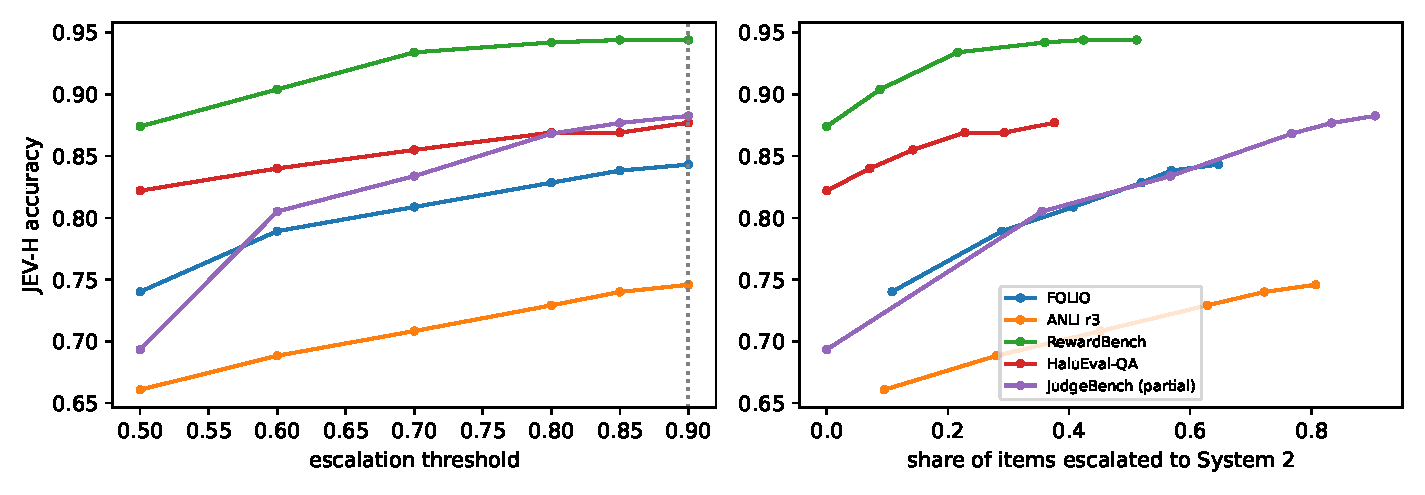
\includegraphics[width=\linewidth]{figures/threshold.pdf}
\caption{JEV-H as the escalation threshold varies (exploratory; the preregistered threshold is 0.90, dotted). Left: accuracy against threshold. Right: accuracy against the share of items escalated to System~2.}
\label{fig:threshold}
\end{figure}
The preregistered threshold of 0.90 was fixed a priori; Figure~\ref{fig:threshold} shows what lower thresholds would have bought, using the System~2 answers already collected.
Most of the gain arrives early: on RewardBench a threshold of 0.70 reaches 93.4\% while escalating 22\% of items (0.90: 94.4\% at 51\%), and on JudgeBench 0.60 already lifts accuracy from 69.3\% to 80.5\% at 36\% escalation.
On FOLIO and ANLI the curve keeps rising to 0.90, because the one-pass model is unsure on most items.
A deployment should choose its threshold from this curve on its own labelled data; \texttt{jevstudy judge} reports it.
